\documentclass[]{article}
\usepackage{fontspec} % compile w/XeLaTeX
\usepackage{lmodern}
\usepackage{setspace} % ability to set the line spacing
\usepackage[fontsize=13]{scrextend}
\usepackage[a4paper, tmargin=0.79in, left=1.38in, right=1.38in,bmargin=1.18in]{geometry}
\usepackage{fancyhdr, graphicx, lastpage}
\usepackage{amsmath}
\usepackage{bm}
\usepackage{caption}
\usepackage{subcaption}
\usepackage{ragged2e}
\usepackage{graphicx}
\usepackage{float}
\usepackage{matlab-prettifier}
\usepackage{pdfpages}
\usepackage{cleveref}
\usepackage{verbatim}
\usepackage[title]{appendix}
\usepackage[sorting=none, backend=biber, style=ieee]{biblatex} 
\addbibresource{Thesis.bib}
\setcounter{secnumdepth}{4}
\usepackage[labelsep=period]{caption}
\captionsetup[table]{name=Table}
\renewcommand{\thetable}{\Roman{table}}
\makeatletter
\def\input@path{"./MATLAB Software"}
\makeatother
\graphicspath{{./figures/}}
\graphicspath{{./images/}}
\allowdisplaybreaks
\usepackage[parfill]{parskip} %Change indents to line breaks between paragraphs
\usepackage[acronym, style=super, nonumberlist]{glossaries}
\emergencystretch=1em % Used to make badness error for bibliography go away

\newacronym{CM}{CM}{Condition Monitoring}
\newacronym{PM}{PM}{Predictive Maintenance}
\newacronym{RMS}{RMS}{Root Mean Square}
\newacronym{SNR}{SNR}{Signal to Noise Ratio}
\newacronym{THD}{THD}{Total Harmonic Distortion}
\newacronym{SINAD}{SINAD}{Signal-to-noise and Distortion Ratio}
\newacronym{TSS}{TSS}{Total Sum of Squares}
\newacronym{SSR}{SSR}{Sum of Squared Regression}
\newacronym{PCA}{PCA}{Principal Component Analysis}
\makenoidxglossaries

\newcommand{\appendixpagenumbering}{
  \break
  \pagenumbering{arabic}
  \renewcommand{\thepage}{\thesection\arabic{page}}
}

\begin{document}
\setmainfont{Perpetua}
\setstretch{1.15}

\includepdf[]{Coverpage_Barron.pdf}
\setglossarystyle{index}
\newpage
\thispagestyle{empty}
\mbox{}
\newpage
\pagenumbering{roman}

\section*{Acknowledgments}
I would like to thank my supervisors Daniel Rönnow and Oscar Bautista Gonzalez for their guidance and patience. I would like to thank the University of Gävle for offering a Masters Program in Electronics and Automation available to take as distance education. I would like to thank Alleima for providing the data to analyses for this Thesis. I would like to thank my partner, Alex Hamelin, for her support.
\newpage

\section*{Abstract}
% Some general comment on the reasons for the project
The availability of industrial machinery is crucial to any business operating in the manufacturing sector. Mechanical failures halt production and unplanned downtime is disruptive and costly. Small failures can lead to catastrophic failures which exponentially increases downtime and repair costs. Identifying a degradation condition before reaching catastrophic failure is key to maintaining machine availability. On the other hand, one does not want to waste resources performing maintenance when not required. For these reasons a large field of academic work is dedicated to analyzing the health of a machine, predicting it's remaining life and thus preventing failures.

% What the project is about
This thesis analyses a tube straightening machine used in the steel industry with the end goal of implementing a condition monitoring strategy. The data for this project comes from a real world application from a multinational manufacturer of steel products. It was obtained using the existing sensors and data acquisition system. The project serves as a study of the existing infrastructure (available sensors) and it's suitability for implementing a condition monitoring strategy. The work is the first step in a larger study and does not attempt to perform any implementation or fault identification. In a broad sense the aim of the project is to find relationships and patterns in the data that could be varying with time as the machine degrades.

% Outling of project steps
The data consists of twelve channels taken over a two week duration. It is prepossessed to isolate periods where the machine is operating and separated into cycles. Each of these is then further processed to extract time and frequency domain features. The features within each channel are compared with each other using the R\textsuperscript{2} coefficient of determination to find combinations that are correlated. A semi automated process is used to select the feature combinations. The same process is performed between signals for each feature. 

% The conclusions of the project
A number of linear regression models are created based on the results from the correlated features as well as some multivariate models. These are then compared using a FIT metric. Potential clustering of machine states are highlighted based on observations in the feature combinations. The conclusions drawn from this study include identification of relationships between signals, potential non-linear correlations and suggestions for future data collection and analysis going forward.
\clearpage

\setcounter{tocdepth}{3}
\tableofcontents
\newpage

\listoffigures
\listoftables
\newpage

\printnoidxglossary[type=\acronymtype, style=list, nogroupskip=true]
\newpage

%\fancypagestyle{plain}{
%	\fancyhf{}
%	%\addtolength{\headwidth}{.5cm}
%	%\addtolength{\headwidth}{.5cm}
%	\fancyhead[C]{Data Analysis for Predictive Maintenance of a Straightening Machine in the Steel Industry}
%	\cfoot{\thepage}
%}
%\pagestyle{plain}
%\setlength{\headheight}{29pt}

\pagenumbering{arabic}
\section{Introduction}
\subsection{Background}
% What is condition monitoring
Condition monitoring (\gls{CM}) is the process of predicting machine health through a combination of sensor data and software algorithms. Sensors measure parameters (vibration, temperature, acoustic emissions etc.) which provide inputs to an algorithm that outputs health metrics. This allows operators to gain an under
ing of when a machine is likely to fail and instead perform some preventative interventions. The ability to monitor equipment health and predict remaining lifetime has valuable benefits. Avoiding unplanned downtime, especially catastrophic failures, allows the extraction of more value from existing resources and less disruption to production schedules.

% Discuss why CM is important
The application of \gls{CM} and \gls{PM} is a large area of research in the machine and manufacturing sector. Of course it is not only limited to machines, being utilized on other engineering structures like bridges~\cite{buckley2023feature}, large process plants like in the oil and gas industry~\cite{telford2011condition} and also biological systems~\cite{tolocsi2011classification}. 
% Discuss more specifically bearing vibration analysis
A common application of \gls{CM} and \gls{PM} in manufacturing is the vibration analysis of rotating machines~\cite{tiboni2022review, kateris2014machine}. Breakdowns in these types of machines are most commonly caused by failures in bearing subsystems. The degradation of a bearing results changes in the vibration signal, among others, which can be a indicator of bearing health and remaining life~\cite{zhang2016degradation}. 

%Even more specifically a tube straightening machine
One such example of an industrial machine that uses roller bearings is a rotary tube straightening machine. These are used as a finishing process in the steel industry for the manufacturing of metal tubes. They are crucial for straightening the tube in the longitudinal direction and improving ovality of the product. 
% Explain why condition monitoring would be useful for a straightening machine
Straightening machines, like many other industrial machines, are expensive to procure and down time is costly. Performance may also be impacted by the machine being in poor condition and in need of maintenance. Thus it is in the interest of the operators to be able to schedule planned maintenance instead of having unplanned downtime and catastrophic failures.

% Challenges for CM
%Advantage of having access to this data
While there is a vast array of research around bearing vibration and \gls{CM}, all machines have their nuances so one \gls{CM} strategy is not necessarily suitable for all. No research specifically involving \gls{CM} on a straightening machine could be found. Unlike a simulation study, \gls{CM} requires real-world data which is not always readily available unless employed by the company owing the machine. This study assesses real world data from such a machine at a Swedish steel manufacturer, Alleima.

% Big Data -> What is Feature Extraction
One of the challenges in implementing \gls{CM} is that there are often huge amounts of data to process and sift through. Thus Feature extraction can be used to reduce the amount of the data whilst preserving the information. By analyzing the features one can then select the most relevant channels and reduce the dimensionality of the data by removing irrelevant, highly correlation or noisy signals. There exist many automated and non-automated methods to select the best features and is a current area of research. This study uses a semi-automated method using the R\textsuperscript{2} correlation coefficient to select the most appropriate features.

% Supervised vs Unsupervised learning
Supervised learning uses labeled data to perform classification, i.e. data is labeled as normal or fault condition. Another difficulty with \gls{CM} research is the limited access to failure data meaning one is often forced to implement unsupervised learning methods. Often one only have partially labeled or totally unlabeled data and thus a different set of techniques exist for unsupervised learning. Here the data analysis is geared towards pattern recognition and clustering since no failure data is available to go with the data. This study has no access to fault or maintenance data and has the goal of trying to find patterns in the data, identify potential clustering opportunities and look at potential trends over time.

\subsection{Project Aim}
The aim of this project is to examine the existing data available for a tube straightening machine and make some observations as to whether it is possible to perform \gls{CM} and/or remaining life analysis for this machine. The first step is to analyze the available data that can be be attained using the existing sensors and data acquisition system. The end goal is to begin developing a strategy that will assist the company to know when the machine requires maintenance. The specific goals of this project are summarized as follows:
\begin{itemize}
\item Understand what signals are related to each other.
\item Understand the signals from a statistical point of view.
\item Calculate signal features and identify which are of significance and which are not useful for condition monitoring i.e. which features may represent degradation condition.
\item Combine appropriate features to create data models and identify trends.
\end{itemize}
\clearpage  
\section{Theory}
\subsection{System}
Rotary straightening machines, \cref{StraighteningMachines,straighteningImage6}, are a type of finishing machine developed to straighten and improve ovality of a metal pipes and tubes. A tube is fed through a series of roller pairs and undergoes a sequence of bending moments which induced controlled plastic deformations. Tubes are subjected to two types of straightening forces, pressure straightening and bend (or offset) straightening. Hydraulic actuators are used to precisely position the height of the rollers and at least some of the rollers are driven by motors which grip and rotate the tube while feeding it through the machine. A number of different configurations for this type of machine exist with six and 10 rolls being common. 

The profile of the rollers is not the same as the tube radius but are hyperbolic in shape and only contact the tube in 3 places. This shape allows it to accommodate different tube diameters by adjusting the gap or height between the upper and lower rollers as well as the angle between them and the tube. The rollers can be adjusted from parallel to the pipe up to approximately 45 degrees, with the upper rollers being adjusted in opposite angle to lower rollers.

Modern straightening machines are equipped with sensors that monitor the amount of force being applied, the deformation of the tube, and other relevant parameters~\cite{zhang2010study}. This feedback allows the machine to make real-time adjustments to the straightening process for optimal results. These sensors, while controlling the process itself can also be used for condition monitoring purposes. Significant research exists on the mechanical analysis of such machines~\cite{kato2014straightening, ma2020effect, ma2021analysis, yu2018theoretical, das1991mechanics, yoshimura2009effect, zhang2019modeling} however no studies relating to condition monitoring of such systems using real life data could be found.

\begin{figure}[H]
    \centering
		\begin{subfigure}{.4\textwidth}
		  \centering
    			\includegraphics[width=.9\linewidth]{straightening2.png}
			\caption{Straightening machine roller profile~\cite{ma2021analysis}}
			\label{straighteningImage2}
		\end{subfigure}%
		\begin{subfigure}{.55\textwidth}
		  \centering
 		   	\includegraphics[width=.9\linewidth]{straightening3.jpg}
			\caption{10 roller straightening machine layout~\cite{zhang2019modeling}}
			\label{straighteningImage3}
		\end{subfigure}
    \caption{Diagrams of straightening machines}
    \label{StraighteningMachines}
\end{figure}

\begin{figure}[H]
	\centering
	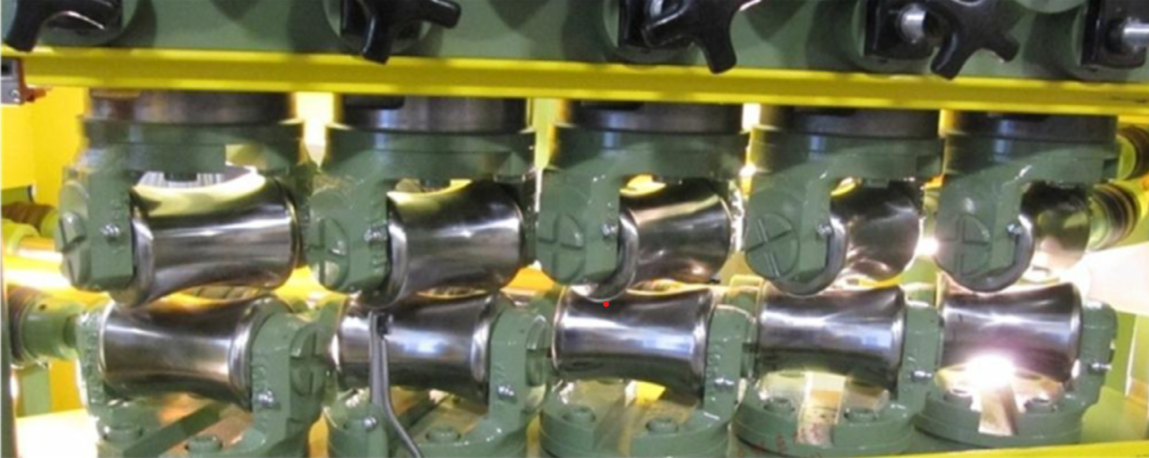
\includegraphics[width=\textwidth, keepaspectratio]{Straightening6.png}
	\caption{Image of a 10 roller straightening machine~\cite{zhang2019modeling}}
	\label{straighteningImage6}
\end{figure}

\subsection{Feature Extraction}
%Why Feature Extraction?
Machine learning algorithms suffer from high amounts of data and information redundancy while requiring vast amounts of storage. Feature extraction, the process of computing numerical values from raw signals, is one method that can be used to combat these issues. By extracting signal features and deciding which are irrelevant one can reduce the amount of data that needs to be stored and processed while still retaining the essence of the signals.

%Feature extraction used in condition monitoring/degradation
Feature extraction techniques are commonly used to estimate degradation trends in machines~\cite{caesarendra2017review,adams2017comparison,hong2014condition}.
%Types of features
Features can include time domain, frequency domain, time-frequency domain (temporal) and model based methods~\cite{teti2010advanced}. Some of the most widely used and effective time domain indicators are mainly based on rms value, the crest factor, and kurtosis~\cite{soualhi2021novel}. Time-frequency values are three dimensional features which include wavelet analysis, spectrograms, scalograms, Wigner-Ville distribution, and kurtograms~\cite{soualhi2021novel}.~\cite{d2019physical} proposes a feature set built on experimental data from sensors plus results from building a simplified kinematic and dynamic model.

Machine \gls{CM} can utilize various form of sensors and signals including: vibration monitoring, acoustic emission monitoring, a fusion of vibration and acoustic, electric motor current monitoring, oil analysis, thermography~\cite{ahmed2020condition}. There is no one size fits all when it comes to condition monitoring. For example a for a slewing bearing, a large low-speed heavy-load bearing, vibration signal is insufficient~\cite{wang2016multiple} and thus fusion models based on torque, temperature and vibration are needed.

\subsection{Time Domain Features} 	
A non exhaustive list of features used for this project are as follows:
\subsubsection*{Mean}
The mean, $ \bar{x} $, is the average value of the signal,
\begin{equation}
\bar{x} = \frac{\sum^N_{i=1} x_i}{N},
\end{equation}
where $ x_i $ is the $ i $:th element of the signal and $ N $ is the number of samples in the signal.
\subsubsection*{Standard Deviation}  
The standard deviation, $\sigma$, is the square root of variance, and measures the dispersion of a data set relative to its mean,
\begin{equation}
	\sigma = \sqrt{\frac{\sum^N_{i=1}(x_i-\bar{x})^2}{(N-1)}}.
\end{equation}
\subsubsection*{\gls{RMS}}
\gls{RMS} is the square root of the mean squared,
\begin{equation}
x_{RMS} = \sqrt{\frac{1}{N} \sum^N_{i=1}x^2_i}.
\end{equation}
Excessive variation in the rms level usually means a change in health status and possible failure. 
\subsubsection*{Shape Factor}
Shape factor is the root mean square divided by the mean of the absolute value,
\begin{equation}
x_{SF} = \frac{ x_{RMS} }  {\frac{1}{N}\sum^N_{i=1}|x_i|}.
\end{equation}
It is dependent on the signal shape and independent of the scale of the signal.
\subsubsection*{Kurtosis}
Kurtosis is derived from the statistical moment of order 4 and is defined as the ratio between the mean value of the signal raised to the power of 4 and the square of its variance, \begin{equation}
x_{kurt} = \frac{\sum^N_{i=1}(x_i-\bar{x})^4}{(N-1)\sigma^4}.
\end{equation}
It is a statistical quantity used to analyze the flattening of a distribution and therefore to observe the shape of the signal. It is a statistical measure of the tailedness of a distribution and indicates the total degree of outliers present. An increase in the number of outliers, and thus an increase in the Kurtosis, can be a indication of an impending fault. For normal bearing operation, kurtosis is close to 3 and increases rapidly with failure.
\subsubsection*{Skewness} 
A measure of asymmetry of the probability density function,
\begin{equation}
x_{skew} = \frac{\sum^2_{i=1}(x_i-m)^3}{(N-1)\sigma^3}.
\end{equation}
Faults can sometimes be revealed through asymmetric distribution.
\subsubsection*{Peak Value}
The maximum value of a signal,
\begin{equation}
x_p = \textrm{max}(x_i),
\end{equation}
where $x_p$ is the peak value of a signal.
\subsubsection*{Impulse Factor} 
The maximum absolute value divided by the mean of absolute value,
\begin{equation}
x_{IF} = \frac{x_p}{\frac{1}{N}\sum^N_{i=1}|x_i|},
\end{equation}
in other words a comparison of the height of the peak to the average value.
\subsubsection*{Crest Factor} 
Crest Factor is found by dividing the maximum absolute value of a signal by the \gls{RMS} value,
\begin{equation}
x_{crest} = \frac{x_p}{\sqrt{\frac{1}{N}\sum^N_{i=1}x^2_i}}.
\end{equation}
Faults can often be detected as a peakiness of signals before they become evident in the energy (\gls{RMS}). Other indicators have been developed based on the crest factor, such as the K-factor, by multiplying the peak value by the rms value or the peak-to-peak value, measuring the difference between the amplitudes of the upper and lower peaks~\cite{soualhi2021novel}.
\subsubsection*{Clearance Factor} 
Clearance factor is the defined as the peak value divided by the squared mean value of the square roots of the absolute values,
\begin{equation}
x_{clear} = \frac{x_p}{(\frac{1}{N}\sum^N_{i=1}\sqrt{|x_i|})^2}.
\end{equation}
For a healthy bearings this feature is maximum and decreases as faults develop.
\subsubsection*{\gls{SNR}}
Ratio of signal power to noise power in decibels,
\begin{equation}
	SNR = 10 \textrm{log}_{10} \frac{P_{signal}}{P_{noise}},
\end{equation}
where $P$ is the average power of the signal and noise. It is usually is expressed as decibels.
\subsubsection*{\gls{SINAD}}
Ratio of total harmonic component power to fundamental power.
\begin{equation}
	SNR = 10 \textrm{log}_{10} \frac{P_{signal} + P_{noise} + P_{distortion}}{P_{noise} + P_{distortion}}, 
\end{equation}
where $P$ is the average power of the signal, noise and distortion and is expressed as decibels.
\subsubsection*{\gls{THD}}
Ratio of total signal power to total noise-plus-distortion power,
\begin{equation}
	THD = \frac{\sqrt{V^2_{h2} + \hdots + V^2_{hN}}}{V_1},
\end{equation}
where $V_N$ is the signal's $N$:th harmonic.
\subsubsection*{Coefficient of Determination}
The coefficient of determination, or $R^{2}$ correlation, is a measure of how well a model predicts the actual output values. It is calculated as the one minus the \gls{SSR} divided by \gls{TSS},
\begin{equation}
R^{2} = 1 - \frac{\textrm{SSR}}{\textrm{TSS}} = 1 - \frac{\Sigma(y_i - \hat{y_i})^2}{\Sigma(y_i - \bar{y_i})^2}. 
\end{equation}
An $R^{2}$ value of 1 means that the two signals are perfectly linear and a value of zero means there is no linear relationship. A value between 0 and 1 indicates some degree of linear relationship exists with the degree of linearity increasing with the value.
\subsection{Frequency Domain Features}
In order to computer the frequency features one must first compute a power spectrum. Matab uses the command, 'findpeaks', to locate the maximum values of the power spectrum.
\subsubsection*{Band Power}
The band power is the area beneath the graph, within a selected frequency range, of the power spectral density vs the frequencies.
\subsubsection*{Peak Amplitude}
Peak amplitude is the height of the frequency with the highest amplitude on the power spectrum.
\subsubsection*{Peak Frequency}
Peak frequency is the value of the frequency which has the highest peak. Matlab uses the command, trapz, to compute the approximate integral of the signal via the trapezoidal method with unit spacing.

%        [peakAmp,peakFreq] = findpeaks(ps,w/factor,'MinPeakHeight',-Inf, ...
%            'MinPeakProminence',0,'MinPeakDistance',0.001,'SortStr','descend','NPeaks',1);
%        peakAmp = [peakAmp(:); NaN(1-numel(peakAmp),1)];
%        peakFreq = [peakFreq(:); NaN(1-numel(peakFreq),1)];
%
%        % Extract individual feature values.
%        PeakAmp1 = peakAmp(1);
%        PeakFreq1 = peakFreq(1);
%        BandPower = trapz(w/factor,ps);
        
\subsection{Feature Selection}
Once features have been calculated the challenge is to isolate the most useful and relevant features. Often data sets contain irrelevant, highly correlated or noisy features that can be removed without a significant loss of information. Ideally non-informative and redundant features are removed to reduce complexity, making models easier to interpret. To this point~\cite{tolocsi2011classification} argues that several widely used classification algorithms can generate misleading feature rankings when the training datasets contain large groups of correlated features. Considering all the research, there is no consensus on which feature/combination of features are best suited for the identification of and distinguishing between faults. 

%Techniques for selecting features
% Best subset selection (forward/backward step-wise selection)
A common method for selecting the most suitable features is forward or backward step wise selection~\cite{james2013introduction}. Forward selection begins with a null model and creates simple linear regressions for each feature on it's own and the model with the lowest RSS is selected. Using that model as a starting point for the next stage another variable is added to create a number of 2 variable models with the lowest RSS being selected to more forward. This process is continued until some stopping rule is satisfied.

% PCA
\gls{PCA} appears to be another popule technique used in feature selection. In one paper, PCA is used to fuse multiple features in order to obtain a bearings state~\cite{lu2016degradation}. Another study uses a PCA-based approach to selecting the most representative features for the classification of defective components and defect severity in three types of rolling bearings~\cite{malhi2004pca}. 

Among other techniques~\cite{buckley2023feature} uses recursive feature elimination and feature correlation clustering, the latter involves using thresholds and removing highly correlation features. This study,~\cite{zhang2016degradation}, proposes a goodness metrics of fit which is a combination of correlation, monotonicity and robustness for feature selection.

%Acoustic emission signals were extracted both by discrete wavelet decomposition and autoregressive modeling. The three feature selection methods include the sequential forward floating selection, and two ant colony optimization-based feature selection methods~\cite{liao2010feature}.

\subsection{Linear Regression Models}
Once a subset of features has been settled upon one can create a linear model. By plotting one signal feature against another signal feature relationships in the data can be revealed. Not only linear relations but quite possibly non-linear relationships too. Calculating a linear regression model is done using linear least squares, 
\begin{equation} \label{eq:reqression}
	\hat{\boldsymbol{\theta}} = (\mathbf{X}^T \cdot \mathbf{X})^{-1} \cdot \mathbf{X}^T \cdot \mathbf{Y},
\end{equation}
where $ \hat{\boldsymbol{\theta}} = \begin{bmatrix} \hat{\theta_{1}} \\ \vdots \\ \hat{\theta_{n}} \end{bmatrix} $, $ \mathbf{X} = \begin{bmatrix} x_{1}(1) & \hdots & x_{k}(1) \\ \vdots & \ddots & \vdots \\ x_{1}(n) & \hdots & x_{k}(n)  \end{bmatrix}$ and 
$ \mathbf{Y} = \begin{bmatrix} y(1) \\ \vdots \\ y(2)\end{bmatrix}$.\\
Equation \ref{eq:reqression} is used for multivariate models as well a two variable models. Once a model has been calculated a normalized goodness of fit function can be used to assess the accuracy of the model,
% Fit equation from compare function
\begin{equation}
	\textrm{Fit Value} = 100 \times \frac{ 1 - \lVert\mathbf{Y} - \mathbf{\hat{Y}}\rVert } { \lVert \mathbf{Y} - \mathbf{\bar{Y}} \rVert }.
\end{equation}
\subsection{Classification and Clustering}
In a perfect world, data would be available for every kind failure mode possible on a machine. If this were true, supervised learning could be used to train an algorithm to recognize all kinds of degradation conditions and faults. One could building a model that predicts or estimates degradation metrics quite easily based on one or more inputs. This is obviously often not the case and a more likely situation is where a number inputs or parameters exists but no quantitative outputs. However, one can still learn about the relationships between signals and the structure from such data using unsupervised learning. The aim here is to identify patterns in the input-output signals from unlabeled data. Thus, it is useful for modeling complex data for which prior knowledge is hard to get~\cite{martin2017unsupervised}.

Unsupervised learning is more of an inference task rather than prediction. Techniques such as auto-encoders, K-means clustering and sparse coding are used to find clusters and patters. Once feature models have been created, one can often find different clustering of data when a machine is in a degraded condition compared to a healthy state.

%Often we are forced to do unsupervised learning since we don't have failure data
Many studies are performed in the lab on specially constructed test rigs which are built to run until destruction~\cite{soualhi2021novel, wang2016multiple, d2019physical, malhi2004pca}. This is not possible on an operational asset since a company cannot afford to run the machine until it fails which. For this reason studies into \gls{CM} of real life machines are often forced to implement unsupervised learning as opposed to supervised.

\begin{comment}
These references haven't been used yet.

A new feature extraction approach using improved symbolic aggregate approximation for machinery intelligent~\cite{zhang2019new}

Automatic feature extraction and selection for condition monitoring and related datasets~\cite{schneider2018automatic}

Comparison of automated feature selection and reduction methods on the condition monitoring issue~\cite{de2018comparison}

Condition monitoring method for the detection of fault graduality in outer race bearing based on vibration-current fusion, statistical features and neural network~\cite{saucedo2021condition}

This paper talks about "top sensitive features" [Feature extraction, condition monitoring, and fault modeling in semiconductor manufacturing systems]~\cite{bleakie2013feature}.

Features selection procedure for prognostics: An approach based on predictability [Features selection procedure for prognostics, an approach based on predictability]~\cite{javed2012features}

Heterogeneous feature models and feature selection applied to bearing fault diagnosis~\cite{rauber2014heterogeneous}

Multifeatures fusion and nonlinear dimension reduction for intelligent bearing condition monitoring~\cite{guo2016multifeatures}

Optimal symbolic entropy: An adaptive feature extraction algorithm for condition monitoring of bearings~\cite{li2023optimal}

"This paper addresses this issue with an application to tool condition monitoring in
milling, where classifiers based on support vector machines and random forest were employed."~\cite{assafo2023stability}
\end{comment}
\clearpage
  
\section{Data Processing}
\subsection{Description of Data}
The data provided by Alleima consists of approximately a one hour period of data each day over a 15 day duration. It is assumed that it was taken from the same period of time each day. The data was captured by an Iba-DAQ data acquisition system with a sampling time 0.02 seconds. The list of signals provided are shown in Table \ref{signalNames}.
\begin{center}
\captionof{table}{Signal Names}\label{signalNames}
\begin{tabular}{ |c|c|l| }
 \hline
Signal Index & Signal Number & Signal Name \\ 
 \hline
1 & 21:07 & Angle over Rolls [deg] \\
 \hline
2 & 21:10 & Position over Rolls [mm] \\
 \hline
3 & 21:12 & Actual moment over Rolls [Nm] \\
 \hline
4 & 21:17 & Angle under roll [deg] \\
 \hline
5 & 21:20 & Actual moment under Rolls [Nm] \\
 \hline
6 & 21:28 & Vibration measurements [mm/s] \\ 
 \hline              
7 & 21:31 & Width position [mm] \\
 \hline
8 & 21:32 & Height position [mm] \\
 \hline
9 & 21:33 & Error position for height [mm] \\
 \hline
10 & 21:34 & Error position for the width [mm] \\
 \hline
11 & 21:35 & Set point force [kN] \\
 \hline
12 & 21:36 & Actual force [kN] \\
 \hline
\end{tabular}
\end{center}

\subsection{Pre-processing}
State detection for this application is performed using Signal 5: 21:20 Actual moment under Rolls. When the machine is not actively processing a tube this value is much less than when it is processing a tube. When no tube is in the system there is none or minimal torque on this sensor and when processing it experiences a much larger moment.
The data is separated into cycles using this signal to isolate the periods where the machine is in the act of processing a part. A threshold of 600 was used as the threshold and a threshold of 500 samples, 10 seconds, was used to filter out short pulses which aren't believed to be full cycles.

\Cref{fig:StateDetection} shows the windows that were identified from each file where the 21.20 signal was above the threshold. Two files, B\_30\_03 and B\_04\_04, contained no identified pulses. In total 240 pulses were identified where the 21.20 signal crosses the threshold. Some of these identified pulses were too short and thus believed to be false positives. Any pulse under 500 samples (10 seconds) was removed from the data for the next stage leaving 224 pulses to extract features from.

\begin{figure}[H]
    \centering
    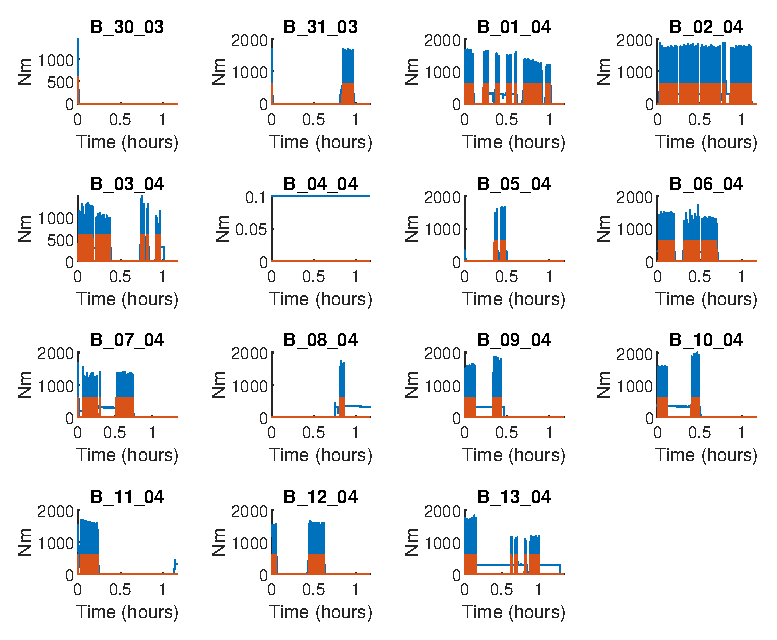
\includegraphics[width=\textwidth, height=\textheight, keepaspectratio]{figures/StateDetectionFig.eps}
    \caption{State detection signal vs 21:20 Actual moment under Rollers}
    \label{fig:StateDetection}
\end{figure}

\Cref{fig:StateDetectionFig_B_02_04} shows one of the plots from \cref{fig:StateDetection}, B\_02\_04, in greater detail. This particular file is the one with the highest number of pulses.

\begin{figure}[H]
    \centering
    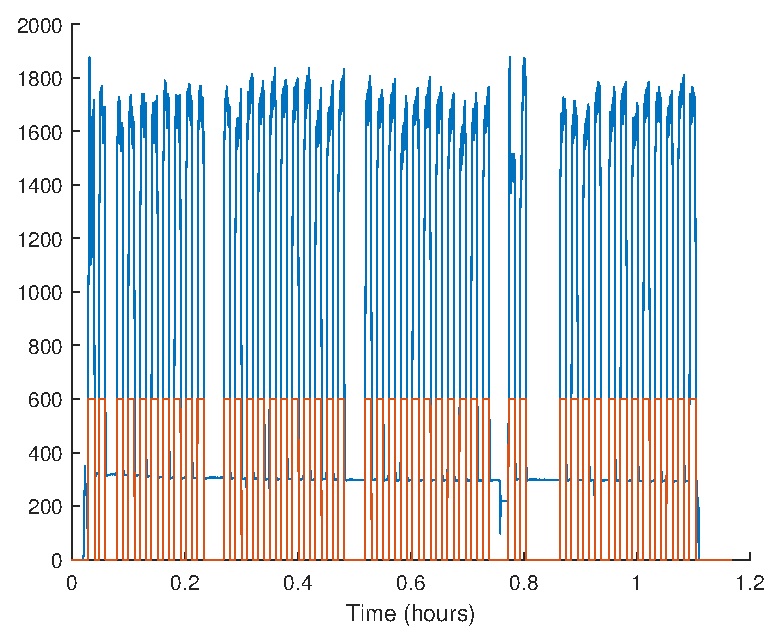
\includegraphics[scale=0.75]{figures/StateDetectionFig_B_02_04.eps}
    \caption{State detection for signal 21:20 performed on file B\_02\_04}
    \label{fig:StateDetectionFig_B_02_04}
\end{figure}

\Cref{fig:IdentifiedPulses} shows pulses or cycles for the signal 21:20 in each of the fifteen files. As mentioned earlier B\_30\_03 and B\_04\_04 show no pulses as all. All the pulses are around 40 seconds in duration with similar shapes but varying profiles.
 
\begin{figure}[H]
    \centering
    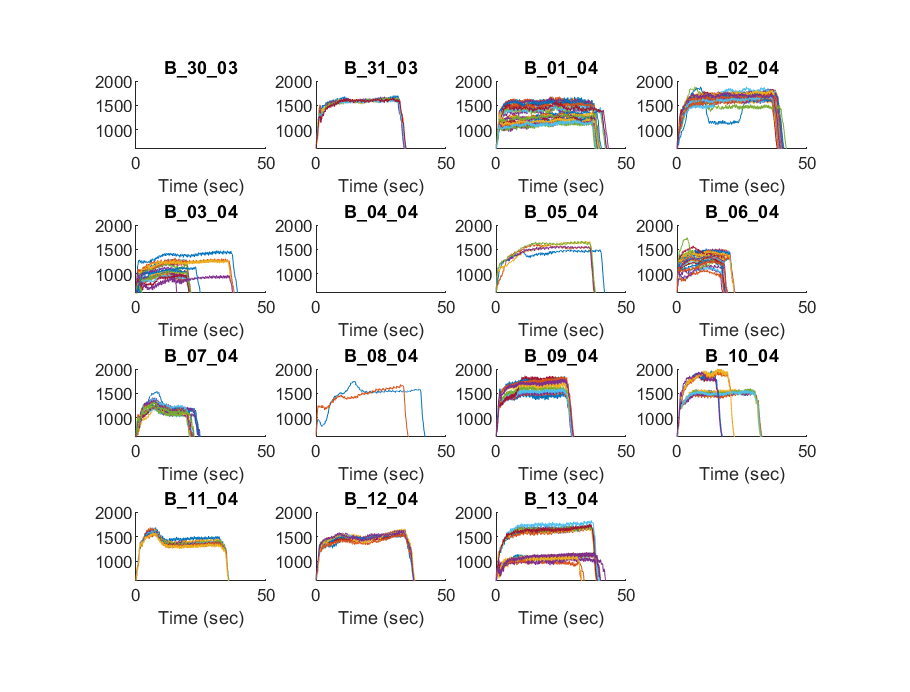
\includegraphics[width=\textwidth, height=\textheight, keepaspectratio]{figures/IdentifiedPulsesFig.eps}
    \caption{Identified pulses in each files for file}
    \label{fig:IdentifiedPulses}
\end{figure}

\Cref{fig:SignalPulses} shows the signals for 224 pulses. Each sensor channel is plotted a different tile. 
\begin{figure}[H]
	\makebox[\textwidth][c]{\includegraphics[width=1.15\textwidth, height=\textheight, keepaspectratio]{figures/SignalPulses.eps}}
    \caption{Signal pulses for 224 pulses on each of the 12 signal channels}
    \label{fig:SignalPulses}
\end{figure}

Using the identified pulses, we can look at all the other signals during the same periods. Signal 1: 21.07 Angle over Rolls and 2: 21.10 Position over Rolls are fairly constant though contain some small deviations. Signal 7: 21:31 Width position and  8: 21:32 Height position are also fairly constant but contain some information when the scale is increased. Signal 21.35 is a fully constant signal and contains nothing but a single value. The label for this signal is set point so it can be assumed that this is a set point that is controlled by the operator and not as sensor on the machine providing feedback. Apart from using this signal for further separating the data into different categories it's likely not that useful for condition monitoring.

\Cref{fig:SignalPulse5} shows the state detection, Signal 5: Moment under rolls, signal in more detail. Visually one can see these are a type of pulse single with a small amplitude frequency component. Signal 3: Moment over rolls looks like a very similar type of signal. Signals 6, 9, 10 and 11 contain some interesting information that can be used for characterize the machine state.

%\begin{figure}[H]
%    \centering
%    \includegraphics[scale = 0.75, keepaspectratio]{figures/SignalPulse1.eps}
%    \caption{Signal 1 Pulses 21:07 Angle over Rolls (deg)}
%    \label{fig:SignalPulse1}
%\end{figure}
 
 
%\begin{figure}[H]
%    \centering
%    \includegraphics[scale = 0.75, keepaspectratio]{figures/SignalPulse3.eps}
%    \caption{Signal 3 Pulses 21:12 Actual moment over Rolls (Nm)}
%    \label{fig:SignalPulse3}
%\end{figure}

\begin{figure}[H]
    \centering
    \includegraphics[scale = 0.75, keepaspectratio]{figures/SignalPulse5.eps}
    \caption{Signal 5 Pulses 21:20 Actual moment under Rolls}
    \label{fig:SignalPulse5}
\end{figure}


%\begin{figure}[H]
%    \centering
%    \includegraphics[scale = 0.75, keepaspectratio]{figures/SignalPulse6.eps}
%    \caption{Signal 6 Pulses 6 21:28 Vibration measurements (mm/s)}
%    \label{fig:SignalPulse6}
%\end{figure}

 
%\begin{figure}[H]
%    \centering
%    \includegraphics[scale = 0.75, keepaspectratio, keepaspectratio]{figures/SignalPulse11.eps}
%    \caption{Signal 11 Pulses 21:35 Set point force (kN)}
%    \label{fig:SignalPulse11}
%\end{figure}

\section{Results}
\subsection{Signal Correlations}
An analysis of the raw signals was performed using R\textsuperscript{2} value. This was performed for a few select files and not for all due to the time taken to run the scripts. Table \ref{correlationTable} shows the R\textsuperscript{2} value for each pair of signals for the data file 1 with the lower triangle being a replica of the upper triangle.\cref{fig:RawSignalCorrelationsFile1} plots all of the signals against each other with the R\textsuperscript{2} values in the range of 0.2 to 0.9 printed on the plots. One signal that is of interest is Signal 6, 21:28 Vibration Measurements, and two combinations it forms with Signal 3: Actual moment over rolls and Signal 5: Actual moment under rolls. Both these combinations have the same correlation value of 0.88 and when looking at \cref{fig:RawSignalCorrelationsFile1} there appears to be a clear non-linear relationship.

Starting with some basic observations of \Cref{fig:File3_Signal5vSignal6}, there are a few combinations that are extremely linear. Two pairs Are highly correlated which means they contain almost exactly the same information. 1: Signal X, 21:31 Width position and Signal X 21:34 Error position for the width, 2: Signal X, 21:32 Height position and Signal X 21:33 Error position for height. Intuitively this makes sense because the errors are so small ....

Signal X, 21:12 Actual moment over Rolls and Signal X, 21:20 Actual moment under Rolls are also highly linear.

\Cref{fig:File3_Signal5vSignal6} shows more clearly what could be an exponential relationship between the vibrations and the torque values on the upper and lower rollers. This plot, for file 3, is representative of the plots in all the other files. This could be explained by the fact that the larger vibration of the rollers the more torque is experienced or applied by the actuators to keep the rollers in place.

\begin{center}
\captionof{table}{R\textsuperscript{2} values for each signal vs. each other signal}
\begin{scriptsize}
\begin{tiny}\begin{tabular}{|l|c|c|c|c|c|c|c|c|c|c|c|c|}
\hline
&\textbf{07}&\textbf{10}&\textbf{12}&\textbf{17}&\textbf{20}&\textbf{28}&\textbf{31}&\textbf{32}&\textbf{33}&\textbf{34}&\textbf{35}&\textbf{36}\\\hline
\textbf{07}&1.00&0.00&0.00&0.00&0.00&0.00&0.00&0.00&0.00&0.00&0.00&0.00\\\hline
\textbf{10}&0.93&1.00&0.00&0.00&0.00&0.00&0.00&0.00&0.00&0.00&0.00&0.00\\\hline
\textbf{12}&0.07&0.07&1.00&0.00&0.00&0.00&0.00&0.00&0.00&0.00&0.00&0.00\\\hline
\textbf{17}&0.37&0.44&0.04&1.00&0.00&0.00&0.00&0.00&0.00&0.00&0.00&0.00\\\hline
\textbf{20}&0.07&0.06&0.99&0.03&1.00&0.00&0.00&0.00&0.00&0.00&0.00&0.00\\\hline
\textbf{28}&0.05&0.07&0.88&0.06&0.88&1.00&0.00&0.00&0.00&0.00&0.00&0.00\\\hline
\textbf{31}&0.22&0.26&0.02&0.35&0.02&0.03&1.00&0.00&0.00&0.00&0.00&0.00\\\hline
\textbf{32}&0.20&0.25&0.01&0.32&0.01&0.03&0.99&1.00&0.00&0.00&0.00&0.00\\\hline
\textbf{33}&0.21&0.25&0.01&0.33&0.01&0.03&0.99&1.00&1.00&0.00&0.00&0.00\\\hline
\textbf{34}&0.22&0.26&0.02&0.35&0.02&0.03&1.00&0.99&0.99&1.00&0.00&0.00\\\hline
\textbf{35}&-Inf&-Inf&-Inf&-Inf&-Inf&-Inf&-Inf&-Inf&-Inf&-Inf&-Inf&0.00\\\hline
\textbf{36}&0.16&0.20&0.01&0.26&0.01&0.03&0.77&0.79&0.79&0.77&-0.00&1.00\\\hline
\end{tabular}
\end{tiny} 
\end{scriptsize}
\label{correlationTable}
\end{center}

\begin{figure}[H]
    \centering
    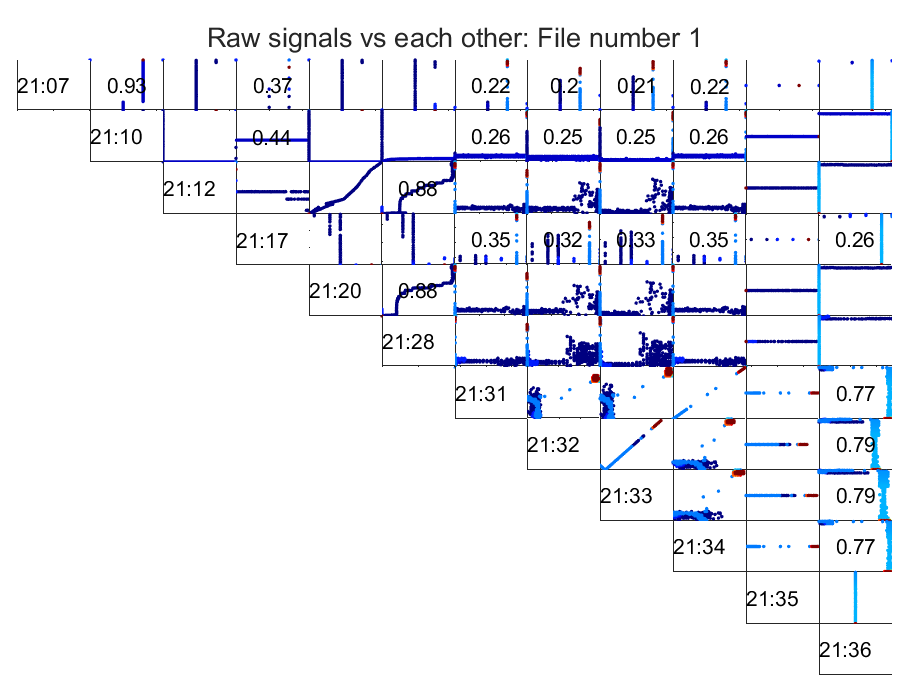
\includegraphics[width=\textwidth, height=\textheight, keepaspectratio]{figures/RawSignalCorrelationsFile1.eps}
    \caption{Plot of each signal vs every other signal with R\textsuperscript{2} values between 0.2 and 0.9}
    \label{fig:RawSignalCorrelationsFile1}
\end{figure}

\begin{figure}[H]
    \centering
    \includegraphics[width=\textwidth, height=\textheight, keepaspectratio]{figures/File3_Signal5vSignal6.eps}
    \caption{Raw data File 3 Signal 5: 21.20 v Signal 6: 21.28 over approximately one hour}
    \label{fig:File3_Signal5vSignal6}
\end{figure}

\subsection{Feature Selection}
Once the data has been pre-processed the feature values are calculated for each identified production cycle. For each channel, the R\textsuperscript{2} value for each pair of signal features is computed and the pairs of data points for each cycle are against each other. This is used as a first stage for filtering out irrelevant data. A small, or zero, R\textsuperscript{2} value indicates that there is a very weak or no linear relationship between that pair of features. On the other hand an R\textsuperscript{2} value of close to 1 indicates that the two features are perfectly or close to perfectly linear. Neither of these feature pairs are of interest as these are not combinations where signals are varying and unlikely to see degradation trends. 

Two threshold values are used to select a range of R\textsuperscript{2} correlated features with this method. An upper and and a lower R\textsuperscript{2} threshold value are specified which reveals feature pairs which are somewhat linear or varying in nature. These are the combinations that are of interest to look for condition indicators.

A semi automatic method can be used to narrow down on feature pairs of interest. An algorithm can cycle through the table of R\textsuperscript{2} values and the features correlated to a number of others can be isolated. Within that combination one can then remove those signals from the group which are highly correlated with each other. Not only can one compare pairs of feature within the same signal but one can also look for relationships between the same feature in varying channels or sensors. 

MATLAB's Diagnostic Feature Designer was used calculate the features from the signal pulse data with Table \ref{signalNames} showing the features that were extracted. Throughout the remainder of the report some figures are labeled with a feature number instead of the full text due to readability and space constraints. Use Table \ref{signalNames} to refer to which feature the indexes represents.

\begin{center}
\captionof{table}{Feature Names}\label{featureNames}
\begin{tabular}{ |c|l|c|l| }
 \hline
 1 & Clearance Factor & 9 & \gls{SINAD}\\
 \hline
 2 & Crest Factor & 10 & Shape Factor\\
 \hline
 3 & Impulse Factor & 11 & Skewness\\
 \hline
 4 & Kurtosis & 12 & Standard Deviation\\
 \hline
 5 & Mean & 13 & \gls{THD}\\
 \hline
 6 & Peak Value &  14 & Band Power \\
 \hline
 7 & \gls{RMS} & 15 & Peak Amplitude 1\\ 
 \hline              
 8 & \gls{SNR} & 16 & Peak Frequency 1 \\
 \hline        
\end{tabular}
\end{center}

\subsection{Feature vs Feature Models}
\Cref{fig:FeatureVsFeatureCombinedSignal6} shows an example of plotting all features against one another for Signal 6: 21:28 Vibration measurements. This was repeated for all signals but just one has been included in the report as an example. Each number on the diagonal represents a feature from Table \ref{signalNames}, starting with the time domain followed by the frequency domain. Only the R\textsuperscript{2} values between 0.3 and 0.8 are printed on the relevant plots. It can be noted that features 1, 2 and 3 all have very straight lines for the plots so here we can say that these features (Clearance, Crest and Impulse Factor), are extremely linear and need only include one of these in any model.
The colors used in these plots are used to represent a pseudo time scale. Although since the data is only from 1 hour per day the color spectrum is not linear however it should be good enough to show a trend over time.


Looking at Feature XXX, it can be seen that the R\textsuperscript{2} value is within the specified range when compared with Features XXX. However when comparing signals within that subset it is clear we realize that XX is highly correlated with XXX thus only one of these is needed for a model since all 3 signals contain the same information. \cref{fig:Models_Signal9Feature7} shows these three remaining features plotted against one another for all cycles. As expected they are somewhat similar in pattern but not exactly the same. Linear regression models were created for Feature 1 Clearance Factor for all three other features but \cref{fig:Models_Signal9Feature7_Linear4} shows.....

\begin{figure}[H]
    \centering
    \includegraphics[width=\textwidth, height=\textheight, keepaspectratio]{figures/FeatureVsFeatureCombinedSignal9.eps}
    \caption{Feature Vs Feature for Signal 9, 21:33 Error position for height}
    \label{fig:FeatureVsFeatureCombinedSignal6}
\end{figure}

\begin{figure}[H]
    \centering
		\begin{subfigure}{.5\textwidth}
		  \centering
    			\includegraphics[width=.9\linewidth]{figures/Models_Signal9Feature7.eps}
		  	\caption{Feature values}
		  	\label{fig:Models_Signal9Feature7}
		\end{subfigure}%
		\begin{subfigure}{.5\textwidth}
		  \centering
 		   	\includegraphics[width=.9\linewidth]{figures/Models_Signal9Feature7_Linear4.eps}
		  	\caption{Linear Model}
		  	\label{fig:Models_Signal9Feature7_Linear4}
		\end{subfigure}
    \caption{Signal 6, 21:28 Vibration measurements Feature 1}
    \label{fig:Models_Signal9Feature7_Caption}
\end{figure}

\begin{figure}[H]
	\captionsetup[subfigure]{justification=Centering}
    \centering
		\begin{subfigure}{.45\textwidth}
		  \centering
    			\includegraphics[width=.9\linewidth]{figures/Models_Signal9Feature11.eps}
		  	\caption{Feature values}
		  	\label{fig:Models_Signal9Feature11}
		\end{subfigure}\hspace{\fill} % maximize horizontal separation
		\begin{subfigure}{.45\textwidth}
		  \centering
 		   	\includegraphics[width=.9\linewidth]{figures/Models_Signal9Feature11_Linear1.eps}
		  	\caption{Linear model}
		  	\label{fig:Models_Signal9Feature11_Linear1}
		\end{subfigure}
		\bigskip
		\begin{subfigure}{.45\textwidth}
		  \centering
    			\includegraphics[width=.9\linewidth]{figures/Models_Signal9Feature11_Linear2.eps}
		  	\caption{Linear model}
		  	\label{fig:Models_Signal9Feature11_Linear2}
		\end{subfigure}\hspace{\fill} % maximize horizontal separation
		\begin{subfigure}{.45\textwidth}
		  \centering
 		   	\includegraphics[width=.9\linewidth]{figures/Models_Signal9Feature11_Linear3.eps}
		  	\caption{Linear model}
		  	\label{fig:Models_Signal9Feature11_Linear3}
		\end{subfigure}
    \caption{Signal 9 21:33 Error position for height Feature 11}
    \label{fig:Models_Signal9Feature11_Caption}
\end{figure}



\begin{figure}[H]
    \centering
		\begin{subfigure}{.5\textwidth}
		  \centering
    			\includegraphics[width=.9\linewidth]{figures/Models_Signal9Feature12.eps}
		  	\caption{Feature values}
		  	\label{fig:Models_Signal9Feature12}
		\end{subfigure}%
		\begin{subfigure}{.5\textwidth}
		  \centering
 		   	\includegraphics[width=.9\linewidth]{figures/Models_Signal9Feature12_Linear1.eps}
		  	\caption{Linear model}
		  	\label{fig:Models_Signal9Feature12_Linear1}
		\end{subfigure}
    \caption{Signal 9 21:33 Error position for height Feature 12}
    \label{fig:Models_Signal9Feature12_Caption}
\end{figure}




\Cref{fig:Models_Signal12Feature1_Caption} shows two relationships of interest. \Cref{fig:Models_Signal12Feature1_Linear1} appears to be a non-linear exponential relationship where the variance is not constant, but increasing as both values move away from 1. \Cref{fig:Models_Signal12Feature1_Linear2} shows a week linear relationship but appears to have two distinct clusters with one on either side of the plot.

\begin{figure}[H]
	\captionsetup[subfigure]{justification=Centering}
    \centering
    
		\begin{subfigure}{.5\textwidth}
		  \centering
    			\includegraphics[width=.9\linewidth]{figures/Models_Signal12Feature1.eps}
		  	\caption{Feature values}
		  	\label{fig:Models_Signal12Feature1}
		\end{subfigure}%
		\begin{subfigure}{.5\textwidth}
		  \centering
 		   	\includegraphics[width=.9\linewidth]{figures/Models_Signal12Feature1_Linear1.eps}
		  	\caption{Clearance vs Shape Factor}
		  	\label{fig:Models_Signal12Feature1_Linear1}
		\end{subfigure}
		
		\bigskip
		
		\begin{subfigure}{.45\textwidth}
		  \centering
 		   	\includegraphics[width=.9\linewidth]{figures/Models_Signal12Feature1_Linear2.eps}
		  	\caption{Clearance vs Skewness}
		  	\label{fig:Models_Signal12Feature1_Linear2}
		\end{subfigure}
		\begin{subfigure}{.45\textwidth}
		  \centering
 		   	\includegraphics[width=.9\linewidth]{figures/Models_Signal12Feature1_Multivariate1.eps}
		  	\caption{Multivariate Model}
		  	\label{fig:Models_Signal9Feature1_Multivariate1}
		\end{subfigure}
		
    \caption{Signal 12 21:36 Actual force}
    \label{fig:Models_Signal12Feature1_Caption}
\end{figure}





\subsection{Signal vs Signal Models}
\Cref{fig:SignalVsSignalFeatureFreq3} shows 
\begin{figure}[H]
    \centering
    \includegraphics[width=\textwidth, height=\textheight, keepaspectratio]{figures/SignalVsSignalFeatureFreq3.eps}
    \caption{Signal Vs Signal for Frequency Domain Feature 3 Peak Frequency 1}
    \label{fig:SignalVsSignalFeatureFreq3}
\end{figure}
\Cref{fig:Models_Feature16Signal3_Linear1} shows the peak frequency of the Actual Moment over Rolls vs Actual moment under Rolls. It can be noted that a majority of the data points follow the a linear model very well. However, a subset of the available data appear to form another linear relationship with a similar gradient but slightly lower intercept.
\begin{figure}[H]
	\centering
	\begin{subfigure}{.5\textwidth}
		\centering
    		\includegraphics[width=.9\linewidth]{figures/Models_Feature16Signal3.eps}
	 	\caption{Feature values}
	  	\label{fig:Models_Feature16Signal3}
	\end{subfigure}%
	\begin{subfigure}{.5\textwidth}
	  \centering
 	   	\includegraphics[width=.9\linewidth]{figures/Models_Feature16Signal3_Linear1.eps}
	  	\caption{Linear Model}
	  	\label{fig:Models_Feature16Signal3_Linear1}
	\end{subfigure}
   	\caption{Feature 16 Peak Frequency 1 Signal 3 Combination 1}
    \label{fig:Models_Feature16Signal3_Caption}
\end{figure}

\subsection{Multivariate Feature Models}

\clearpage 

\section{Discussion}
% In this chapter the results and the chosen method are discussed, as well as the strengths and weaknesses of the work.
% Discuss results - Comments on what signals are related
This study aimed to give suggestions as to what signals and/or signal features are of value for future condition monitoring studies and which ones are not. 

Unsurprisingly the vibration signal is probably the most interesting for finding correlations?????

Of the data provided, many of the signals were relatively constant. In particular, Signal 11, 21:35 Set point force is perfectly constant and is not suitable for condition monitoring. The following signals are not overly useful to condition monitoring as they are fairly constant in mean value and contain little variable: 
1, 21:07 Angle over Rolls
2, 21:10 Position over Rolls
4, 21:17 Angle under roll
7, 21:31 Width position
8, 21:32 Height position

These signals are most useful for condition monitoring:
3 21:12 Actual moment over Rolls
5 21:20 Actual moment under Rolls
6 21:28 Vibration measurements 
9 21:33 Error position for height
10 21:34 Error position for the width
12 21:36 Actual force           

%Comment on Method
Comments include.....

It would be good to inquire with the company about whether what they have provided is the full set of available signals. Temperature and acoustic emissions are also highly effective types of sensors for condition monitoring so if there was in fact additional data these would be of interest. If none of these sensors exist perhaps a good consideration might be to add one or more of these types of measurements to complement existing infrastructure.

%Weaknesses
The data supplied for the project is from a two week period which probably does not give a good insight into the life cycle of the machine. No maintenance data is provided. Perhaps maintenance is only required on a yearly cycle and the machine degradation, thus we are not really getting a get insight into the degradation of the machine over time. Perhaps a better selection of data would include a snippet of data every 1-2 weeks over a year long period and thus one could get a better view of how the machine degrades over a year.

Ideally we would have data over the lifespan of a machine. The data we have right know, we don't know whether is is normal operating data. It could be right at the beginning of the lifecycle or could be just at the end of the machines lifecycle. A system that has been operating for a long period of time will undergo changes due to the natural wear of the system.

%Put in context/comparison with references at the beginning. 
This study....

An analysis of such data can be expanded exponentially but one can only look at so much before moving on. It is also beneficial to, at least begin with, simple things like two variable linear regression.

%Enhance scientific research, upgrade the technological capabilities of industrial sectors in all countries, in particular developing countries, including, by 2030, encouraging innovation and substantially increasing the number of research and development workers per 1 million people and public and private research and development spending.
The subject matter, methods and results used in this report are in good agreement with target 9.5 of the 2030 Agenda for sustainable development\cite{united2015department}. Hopefully this work will upgrade technology capabilities in industrial sectors and will assist workers in the field of research and development. 

\subsection{Future Work}
This report has identified potential clusters based on visual observations in the data. However, no attempts were made to implement any clustering algorithms. This would be the logical next step, to apply some machine learning techniques, in trying to identify degradation states. In particular methods such as K nearest neighbors or K-means clustering approach.

The straightening machine in this study produces products of of different diameters. At least one of the signals can be used to indicate this diameter. This could be used to classify the data further into different tube widths. A suggestion for future studies is to perform an additional prepossessing step to separate data into periods where the machine is producing tubes with certain diameters. Some of the clustering suggestions or relationships given in this study could just be identifying when the machine is producing a tube of a certain width. Separating data and focusing on only one tube width would removed any chance of this. A method like this would have been challenging since only 224 pulses were identified to begin with and thus a further reduction might result in not enough data to make meaningful observations.

Non-linear modelling.....
\clearpage

\section{Conclusion}
%Here the work should be concluded and the major results presented. Suggestions of continuation and spin-off projects may be brought forward, usually under a separate subsection called “Future Work”.
A study of the available data on a steel tube straightening machine was conducted with regards to using the existing infrastructure for condition monitoring.
\begin{itemize}
\item Correlation was performed on the raw signal data to identify relationships between the sensor channels.
\item The data was prepossessed using an amplitude threshold for the state detection and then a time threshold to eliminate false cycles.
\item Time and frequency domain features were extracted from the cycles.
\item For every sensor channel, each feature was plotted against every other feature and the R\textsuperscript{2} correlation coefficient was calculated.
\item An upper and lower threshold, was used to selected a combination of features that are somewhat correlated but not well perfectly correlated.
\end{itemize}
\newpage

\section{References} 
\printbibliography[heading=none] 
\clearpage  

\begin{appendices}
\appendixpagenumbering
\section{Matlab Code}
\UseRawInputEncoding

\lstinputlisting[frame=single, numbers=left, style=Matlab-editor, basicstyle=\ttfamily\scriptsize]{"./MATLAB Software/LoadRawData.m"}

\lstinputlisting[frame=single, numbers=left, style=Matlab-editor, basicstyle=\ttfamily\scriptsize]{"./MATLAB Software/LoadFeatures.m"}

\lstinputlisting[frame=single, numbers=left, style=Matlab-editor, basicstyle=\ttfamily\scriptsize]{"./MATLAB Software/fnStateDetection.m"}

\lstinputlisting[frame=single, numbers=left, style=Matlab-editor, basicstyle=\ttfamily\scriptsize]{"./MATLAB Software/fnPlotFeatureVsFeature_Array.m"}

\lstinputlisting[frame=single, numbers=left, style=Matlab-editor, basicstyle=\ttfamily\scriptsize]{"./MATLAB Software/fnPlotSignalVsSignal.m"}

\lstinputlisting[frame=single, numbers=left, style=Matlab-editor, basicstyle=\ttfamily\scriptsize]{"./MATLAB Software/fnPlotModel.m"}

\lstinputlisting[frame=single, numbers=left, style=Matlab-editor, basicstyle=\ttfamily\scriptsize]{"./MATLAB Software/fnPlotModel3D.m"}

%\lstinputlisting[frame=single, numbers=left, style=Matlab-editor]{"./MATLAB Software/PreProcessData.mlx"}
\preto{\endappendices}{\clearpage}
\end{appendices}
\end{document}